\chapter{Description du capteur}

Les informations relatives aux sportifs sont acquises par le biais du capteur. Il sera composé d’un assemblage de différents éléments déjà existants dans le commerce. On veillera à minimiser au maximum son poids ainsi que sa taille pour éviter de gêner le sportif durant sa course. Une fois assemblé, il sera placé dans une boîte étanche qui disposera d’un bracelet élastique ce qui permettra à l’athlète de le porter facilement. Enfin il doit également disposer de sa propre source d’énergie sous la forme d’une batterie, celle-ci doit lui conférer une autonomie assez grande pour pouvoir fonctionner durant l’entièreté d’une course.

Trois types de données différentes seront récupérées, la position GPS du coureur (longitude/latitude), son rythme cardiaque en battement par minute ainsi que la cadence de ses pas en pas par minute. Régulièrement le capteur va effectuer les acquisitions, puis il va traiter les données et créer un paquet de données. Une fois que le paquet est prêt à être transmis, le capteur utilise son module de transmission LoRa pour les envoyer à la passerelle. Quand ce processus est terminé, le capteur se met en attente jusqu’au début du cycle suivant et recommence le processus. Ce processus est illustré par la figure ~\ref{fig:proc_capteur}.

\begin{figure}[htb]
\centering 
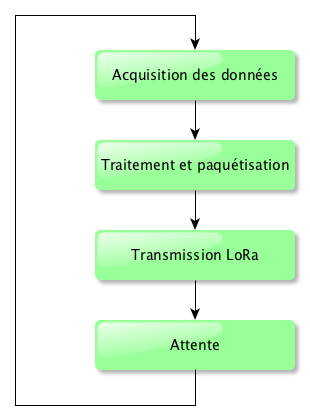
\includegraphics[width=0.4\columnwidth]{../images/capteur_flowchart.png} 
\caption[Processus Capteur]{Processus du capteur}
\label{fig:proc_capteur}
\end{figure}

Le microcontrôleur est la partie centrale du capteur, c’est lui qui exécute le programme d’acquisition des différents paramètres décrit ci-dessus, qui fait le traitement des données pour ensuite les envoyer en utilisant la transmission LoRa. Le cœur du capteur sera donc un module disposant d’un microcontrôleur ainsi que tout ce qui lui ai nécessaire pour fonctionner (oscillateur, mémoire, interfaces…).

Viendront se coupler au microcontrôleur les quatre modules suivants :
\begin{itemize}
\item Un module GPS permettant le positionnement du coureur
\item Un module permettant la mesure du rythme cardiaque
\item Un module accéléromètre qui donnera la possibilité de déterminer la cadence du coureur
\item Un module radio LoRa avec antenne qui se chargera de la communication avec la passerelle\\
\end{itemize}

Le microcontrôleur devra communiquer avec chacun de ses modules d’une manière ou d’une autre afin de pouvoir récupérer les informations et les transmettre. Les modules n’ont pas les mêmes contraintes, il est donc impératif de sélectionner un environnement dans lequel chacun d’eux aura à disposition le canal de communication approprié que ce soit une interface série, un I/O ou un bus SPI par exemple.

Les prochaines sections de ce chapitre décrivent chaque module ainsi que leurs interfaces.

\section{Position GPS}

Un module GPS est responsable de déterminer la position du coureur. Le système GPS se base sur une constellation d’au moins 24 satellites qui sont en orbite moyenne (Altitude de 20'200 km) autour de la Terre. Afin qu’un utilisateur puisse déterminer sa position sur le globe, il est nécessaire qu’il ait la vue sur au moins 4 satellites. A une fréquence très précise, donné par des horloges atomiques, les données de position orbitales ainsi que de temps sont envoyées en direction de la planète, grâce à ses informations le receveur est en mesure de connaître la distance de chacun des satellites en vue et donc de calculer sa position géographique ainsi que de déterminer le temps actuel, c’est ce que l’on appelle le GPS « lock » ou « fix ». \cite{gps_overview}

Cette tâche compliquée est entièrement à la charge du module GPS lui-même, il dispose d’une antenne qui lui permet de recevoir les données envoyées par les satellites, de les analyser et de calculer les informations requises pour les mettre à disposition du microcontrôleur.
La grande majorité des modules GPS transmettent les informations en utilisant une interface série UART sur lequel des messages de type NMEA 0183 sont envoyé vers le récepteur. Ce protocole définit le format de plusieurs messages qui contiennent diverses informations de position, de statuts et de temps. \cite{nmea_0183}

Dans le cadre du projet de Bachelor l’information principale qui sera exploité sera la longitude et latitude du capteur qui permettra de déterminer la position du coureur. D’autres informations intéressantes pourront éventuellement être utilisées comme le temps ou l’altitude.

Le composant peut être directement placé sous l’antenne ou alors il existe également des solutions avec antenne branché par un câble comme montré sur la figure~\ref{fig:antenne_gps}.

\begin{figure}[htb]
\centering 
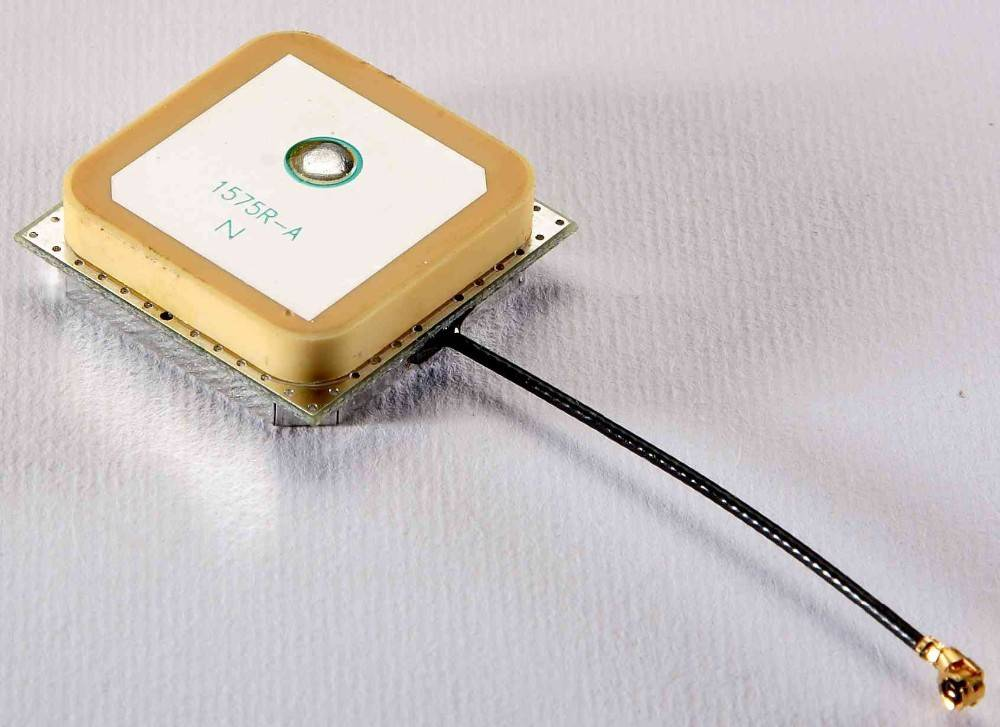
\includegraphics[width=0.6\columnwidth]{../images/active-gps-antenna-large.jpg} 
\caption[Antenne GPS]{Antenne GPS - © SODAQ}
\label{fig:antenne_gps}
\end{figure}

\section{Rythme cardiaque}

Il existe deux moyens principaux de déterminer le rythme cardiaque d’une personne. La première solution consiste à utiliser une ou plusieurs électrodes qui détecteront directement les signaux électriques émit par le cœur, c’est le principe utilisé par les électrocardiogrammes. L’autre solution est basée sur l’utilisation de LEDs placés contre la peau et qui vont émettre de la lumière à une fréquence régulière, la lumière réfléchie par réfraction et qui dépend de la dilatation des vaisseaux sanguins est ensuite détecté par le capteur et permet de déterminer le rythme cardiaque de l’utilisateur. Cette deuxième technique est très utilisée dans les montres GPS utilisés pour le sport car elle a l’avantage de pouvoir être directement intégrée dans le boîtier et ne nécessite que peu de moyen pour être mis en place.

Pour le capteur de ce projet, les deux solutions existent sur le marché, cependant la solution de l’électrocardiogramme semble plus appropriée et pratique car elle permet d’utiliser un cardiofréquencemètre sans fil du commerce et évite ainsi au porteur du capteur de devoir s’accommoder des fils qui sont nécessaire pour le fonctionnement de la solution à base de LED.

Dans les deux cas, l’utilisation par le microcontrôleur est semblable, la sonde sera connectée sur une entrée digitale et elle émettra une impulsion à chaque fois qu’un battement sera détecté. Il suffit donc de compter le nombre d’impulsion et de mesurer le temps pendant lesquels elles ont eu lieu pour pouvoir déterminer la fréquence cardiaque en BPM (Battement par minute).

La formule suivante permet de calculer le rythme cardiaque~$rc$ en battement par minutes (BPM).

\begin{equation}\label{eqn:rythme_card}
rc = \frac{60 * n}{t}
\end{equation}

Avec~$n$ le nombre de battement accumulé pendant un temps~$t$ en secondes.

Les battements du cœur peuvent être détecté grâce à une sangle pectorale munie d’un cardiofréquencemètre. Adafruit propose ce genre de dispositif, il émet une impulsion chaque fois qu'un battement est détecté, un petit module connecté sur une ligne d'entrée du microcontrôleur permet ensuite au logiciel de les compter. Ce type de dispositif est illustré sur la figure~\ref{fig:cardiofreq}. Du fait de la gêne occasionnée par une électrode cette solution sera privilégiée.

\begin{figure}[htb]
\centering 
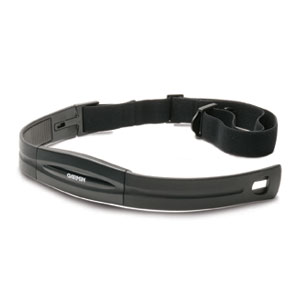
\includegraphics[width=0.6\columnwidth]{../images/garmin-heart-rate.jpg} 
\caption[Sangle Pectorale]{Sangle pectorale - © Garmin}
\label{fig:cardiofreq}
\end{figure}



